\section{Qafny: A High-level Quantum Language Admitted a Proof System}
\label{sec:qafny}

\begin{figure}[t]
{\small
\[\hspace*{-0.5em}
\begin{array}{r l l}
\textcolor{blue}{1}
&
\{A(x) * A(y) \}
\;\;\text{where}\;\;
A(\beta) = \beta[0..n] \mapsto \ket{\overline{0}} 
&
\{x[0..n]: \tnort, y[0..n]: \tnort\}
\\[0.5em]
\textcolor{blue}{2}
& \ssassign{x}{}{\ihadh};\\[0.5em]

\textcolor{blue}{3}
&
\textcolor{teal}{
\{x[0..n] \mapsto \dabs{\ihadh}(\ket{\overline{0}}) * A(y) \}
}
&
\textcolor{teal}{
\{x[0..n]: \thadt, y[0..n]: \tnort\}
}
\\
\textcolor{blue}{4}
&
\textcolor{teal}{
\Rightarrow
\{x[0..n] \mapsto C * A(y) \}
}
\;\;\text{where}\;\;
\textcolor{teal}{
C = \shad{2^n}{n}{}
}
&
\textcolor{teal}{
\{x[0..n]: \thadt, y[0..n]: \tnort\}
}
\\[0.5em]
\textcolor{blue}{5}
& \ssassign{y}{}{y\splus 1};
\\[0.5em]

\textcolor{blue}{6}
&
\textcolor{teal}{
\{x[0..n] \mapsto C * y[0..n] \mapsto \dabs{y\splus 1}(\ket{\overline{0}}) \}
}
&
\textcolor{teal}{
\{x[0..n]: \thadt, y[0..n]: \tnort\}
}
\\[0.5em]
\textcolor{blue}{7}
&
\textcolor{teal}{
\Rightarrow
\{x[0..n] \mapsto C * y[0..n] \mapsto \ket{\overline{0}.1} \}
}
&
\textcolor{teal}{
\{x[0..n]: \thadt, y[0..n]: \tnort\}
}
\\[0.5em]
\textcolor{blue}{8}
& 
\textcolor{teal}{
\Rightarrow
\{ E(0) \}
}
\;\;
\texttt{where}\;\;
\textcolor{teal}{E(k) =}
&
\textcolor{teal}{
\{x[0..n]: \thadt, \{x[0..0],y[0..n]\}: \tcht\}
}
\\[0.2em]
&
\qquad\qquad\quad\;
\textcolor{teal}{
\begin{array}{l}
x[k..n] \mapsto \shad{2^{n \,\sminus\,  k}}{n \,\sminus\, k}{}\;*
\\[0.2em]
\{x[0..k],y[0..n]\} \mapsto \scha{2^k}{\frac{1}{\sqrt{2^k}}}{j}{a^{j}\;\%\;N}
\end{array}
}
\\[0.5em]
\textcolor{blue}{9}
&\sqforh{\sint{j}{0}}{j\,\slt\, n}{x[j]}{\dplus{j}}
\\[0.5em]
\textcolor{blue}{10}
&
\quad\{E(j) \}
&
\{x[j..n]: \thadt, \{x[0..j],y[0..n]\}: \tcht\}
\\[0.4em]
\textcolor{blue}{11}
&
\quad\ssassign{y}{}{a^{2^j}y\;\%\; N};
\\[0.5em]
\textcolor{blue}{12}
&
\textcolor{teal}{
\{E(n) \}
}
&
\textcolor{teal}{
\{x[0..0]: \thadt, \{x[0..n],y[0..n]\}: \tcht\}
}
\\[0.4em]
\textcolor{blue}{13}
&
\textcolor{teal}{
\Rightarrow
\{\{x[0..n],y[0..n]\} \mapsto \scha{2^{n}}{\frac{1}{\sqrt{2^{n}}}}{j}{a^{j}\;\%\;N} \}
}
&
\textcolor{teal}{
\{\{x[0..n],y[0..n]\}: \tcht\}
}
\\[0.4em]
\textcolor{blue}{14}
& \sexp{u}{\smea{y}}{...}
\\[0.4em]
\textcolor{blue}{15}
&
\textcolor{purple}{
\big{\{}
\begin{array}{l}
x[0..n] \mapsto \smch{\frac{1}{\sqrt{s}}}{s}{t\,\splus\,k p} 
\wedge
p = \texttt{ord}(a,N)
\\
\wedge\;
u=(\frac{p}{2^n},a^{t}\;\%\;N)
\wedge
s=\texttt{rnd}(\frac{2^n}{p})
\end{array}
\big{\}}
}
&
\textcolor{purple}{
\{\{x[0..n]\}: \tcht\}
}
\end{array}
\]
}
\caption{Pre-measurement quantum steps of the Shor's algorithm. $\sord{a,N}$ gets the order of $a$ and $N$. $\srnd{r}$ rounds $r$ to the nearest integer. The right-hand-side contains the types for the sessions involved. $\ket{j}$ is an abbreviation of $\ket{\tos{j}}$.
$\tos{j}$ turns a number $j$ to a bitstring. $\overline{0}.1$ is a bitstring concatenation operation. }
\label{fig:shorqafny}
\end{figure}

We designed \qafny, the core language of QNP,
to be able to express quantum programs in terms of
high-level operations that are abstracted away low-level circuit gates.
The operations in \qafny are analogized to classical array 
aggregate operations so that automated verification is feasible.
\qafny's type system tracks the transformation of sessions, 
clusters of possibly entangled qubits and the state unit in \qafny programming,
with three types indicating the qubit clusters' state representations.
The \qafny proof system is designed to capture the quantum to classical array aggregate operation analogies
by utilizing the type system to ensure the session formats in programs and predicates.
All of these features are novel to quantum languages and proof systems. 

\begin{wrapfigure}{r}{8.2cm}
  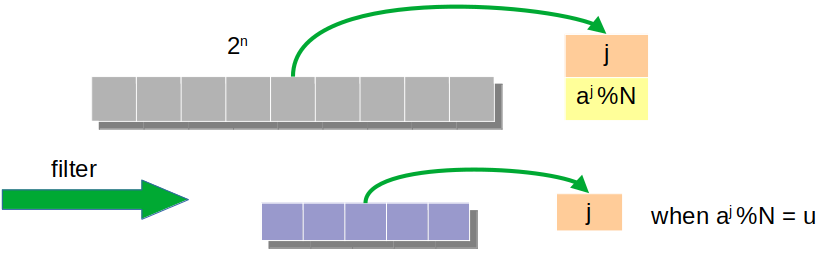
\includegraphics[width=.60\textwidth]{shorsmap}
  \caption{The array analogy of Shor's first half in \Cref{fig:shorqafny}. }
\label{fig:shorsanalog}
\end{wrapfigure}

This section presents \qafny states and the language's syntax, typing, 
semantics, proof system, and soundness/completeness results.  
As a running example, we use the Shor's algorithm~\cite{Shor94} shown in \Cref{fig:shorqafny}. 
Given an integer $N$, Shor's algorithm finds its nontrivial prime factors, which has the following step: (1) randomly pick a number $1 < a < N$ and compute $k=\texttt{gcd}(a,N)$ \footnote{compute the greatest common divisor of $a$ and $N$}; (2) if $k \neq 1$, $k$ is the factor; (3) otherwise, $a$ and $N$ are coprime and we find the order $p$ of $a$ and $N$ \footnote{the order $p$ is the smallest number such that $a^p \% N = 1$}; (4) if $p$ is even and $a^{\frac{p}{2}} \neq -1 \% N$, $\texttt{gcd}(a^{\frac{p}{2}}\pm 1,N)$ are the factors, otherwise, we repeat the process. Step (2) is the quantum part of Shor's algorithm and \Cref{fig:shorqafny} and \Cref{fig:shorqafny2} show its automated proof in QNP. In \Cref{fig:shorexample}, we show the actual implementation and proof in the Qafny tool.

The Shor's pre-measurement quantum steps in \Cref{fig:shorqafny} can be analogized as an efficient array filter operation.
The steps before line 14 (steps at line 2, 5 and 9-11) create a $2^n$-length of pairs, each of which is formed as $(j,a^j \% N)$ where $j\in [0,2^n)$. The measurement in line 14 filters the array as a new one ($x[0..n]$) with all elements $j$ satisfying $a^j \% N=u$ where $u$ is a randomly picked number. Notice that modulo multiplication $f(j)=a^j\%N$ is a periodic function. All elements in $x[0..n]$ satisfy $a^j \% N=u$, which means that 1) there is a smallest $t$ such that $a^t \% N=u$, and 2) all elements can be rewritten as $j=t+kp$ and $p$ is the period of the modulo multiplication function, which is given as the post-condition on the right of line 15.
The implementation and correctness proof in \Cref{fig:shorqafny} exactly reflects the array analogy aspect.
\ignore{
One of the biggest advantage of using \qafny is that we can analogize quantum operations to classical array operations, so that we can utilize the existing automated proof infrastructure in many tools, such as Dafny.
In the Qafny implementation, verifying a quantum program usually requires only the user input of the pre-, post-, and loop invariant. For example, the proof of \Cref{fig:shorqafny} in \qafny requires none of the states marked teal, but only the conditions marked black and purple. \footnote{The purple is also not needed if we combine the Shor's first and second half algorithms together.}
Here, we step by step discuss the states, program syntax, and proofs of the aspect.
}
Notice that only the marked black and purple parts in \Cref{fig:shorqafny} are required to input in the \qafny implementation, and the marked teal parts can be inferred by the \qafny proof system. \footnote{The purple is also not needed if we verify the whole Shor's algorithm in \Cref{fig:shorexample}.}

We first introduce \qafny states, syntax, and type system. Then, we discuss its semantics and proof system and metatheories.

\subsection {Classical and Quantum States}

\begin{figure}[t]
{
  \small
\[\hspace*{-0.5em}
\begin{array}{l}
\textcolor{blue}{\text{Basic Terms:}}\\[0.2em]
\begin{array}{llcl llcl llcl}
\text{Nat. Num} & m, n & \in & \mathbb{N}
&
      \text{Real} & r & \in & \mathbb{R}
&
      \text{Amplitude} & z & \in & \mathbb{C}
\\
      \text{Variable} & x,y &&

 & \text{Bit} & d & ::= & 0\mid 1       
&
      \text{Bitstring} & c & \in & d^{+}      
\\
\text{Phase} & \alpha(r) & ::= & e^{2\pi i r}
\\
\end{array}
\\[1em]
\textcolor{blue}{\text{Modes, Kinds, Types, and Classical/Quantum Values:}}\\[0.2em]
\begin{array}{llclll} 
      \text{Mode} & g & ::= & \cmode  \mid \mmode\\
      \text{Classical Value} & v & ::= & n \mid (r,n)\\
      \text{Kind} & \overline{g} & ::= & g \mid \qmode{n} \\
      \text{Basis}& \beta & ::= & (\ket{c})^+\\
      \text{Quantum Type} & \tau & ::= & \tnort &\mid \thadt & \mid \tcht \\
      \text{Quantum Value} & q & ::= & z\beta & \mid \shad{2^n}{n}{\alpha(r_j)} &\mid \ssum{j=0}{m}{z_j\beta_j} \\
    \end{array}
\\[1em]
\textcolor{blue}{\text{Quantum Sessions, Environment, and States}}\\[0.2em]
\begin{array}{llclcl} 
      \text{Range} & l & ::= & x[n..m] \\
      \text{Session} & \kappa & ::= & \overline{l} & \text{concatenated op} & \uplus \\
      \text{Type Environment} & \sigma & ::= & \overline{\kappa : \tau } & \text{concatenated op} & \cup \\
      \text{Quantum State} & \varphi & ::= & \overline{ \kappa : q } & \text{concatenated op} & \cup \\
    \end{array}
\end{array}
  \]
}
  \caption{\qafny element syntax. Each range $x[n..m]$ in a session $l$ represents the number range $[n,m)$ in a qubit array piece $x$. Sessions are finite lists, while type environments and states are finite sets. the operations after "concatenated op" refer to the concatenation operations for session, type environments and quantum states. $(\ket{c})^+$ is a non-empty list of bases $\ket{c_i}$, and refers to $\ket{c_0}\otimes ... \otimes \ket{c_n}$. }
  \label{fig:qafny-state}
\end{figure}

\qafny has three \emph{kinds} of parameters in \Cref{fig:qafny-state}: a $\cmode$-kind classical integer parameter \footnote{In the \qafny implementation one can utilize any classical typed parameters allowed in Dafny . For simplicity, we only allow integers in this paper.}, a $\mmode$-kind classical integer parameter $(r,n)$ with a probability characteristic $r$ representing the theoretical probability of the measurement resulting in the natural number value $n$, and a $\qmode{n}$ kind quantum parameter, where $n$ represents the number of bits in a qubit array piece. Quantum parameters are classified as three types: $\tnort$, $\thadt$, or $\tcht$, representing the three types of quantum values in \Cref{sec:background}. We have subtyping relations over quantum types, such that $\tnort$ and $\thadt$ are subtypes of $\tcht$, representing the fact that $\tnort$ and $\thadt$ quantum values can be rewritten as $\tcht$-forms. 

\qafny represents qubit arrays as \emph{sessions} ($\kappa$), which consist of different \emph{disjoint ranges}, each of which describes an array fragment $x[n..m]$, where $x$ is a variable representing a qubit array piece and $[n..m]$ represents the array fragment from position $n$ to $m$ (exclusive) in array piece $x$. For simplicity, we assume that there are no aliasing array piece variables in this paper, i.e., two distinct variables represent disjoint array pieces. For example, $\{\{x[0..n],y[0..n]\}$ in \Cref{fig:shorqafny} line 12 represents a $2n$ qubit array containing two disjoint pieces $x[0..n]$ and $y[0..n]$ referring to the ranges $[0,n)$ in groups $x$ and $y$, respectively. We also abbreviate a singleton session $\{x[n..m]\}$ as a range $x[n..m]$.
In \qafny quantum type environments and states, qubit values are always associated with sessions, where a length-$n$ session is associated with a $\tnort$-type state $z\beta$, $\thadt$-type state $\shad{2^n}{n}{\alpha(r_j)}$, or $\tcht$-type state $\ssum{j=0}{m}{z_j\beta_j}$. In the $\tnort$-type or $\tnort$-type state, the lengths $\slen{\beta}$ (or $\slen{\beta_j}$) of every basis $\beta$ (or $\slen{\beta_j}$) \footnote{The length of $\beta$ is defined as the sum of all length of basis bitstrings in $\beta$.} are the same and $\slen{\beta} \ge n$ (or $\slen{\beta_j} \ge n$); in $\thadt$-type state, the session length is the same as the qubit array length $n$.
\qafny type environments and states are finite, and the domain sessions do not overlap, i.e., for all $\kappa, \kappa' \in \dom{\sigma}$ (or $\varphi$), $\kappa \neq \kappa' \Rightarrow \kappa \cap \kappa' = \emptyset$.

\qafny utilize \emph{equivalence relations} over quantum sessions, quantum values and states (as shown in \Cref{fig:qafny-eq}) to facilitate automated program verification, written as $\equiv$ for state equivalence and $\preceq$ for environment partial order. One example is the rewrite from line 12 to line 13 in \Cref{fig:qafny-state}, where the state of session $x[0..0]$ is rewritten to $\texttt{true}$, because the session is essentially empty.
The common equivalence relations are state form rewrites, permutations, split and joins. 
State rewrites are to transform state forms, such as the rewrite of session $\{x[0..0],y[0..n]\}$ from type $\tnort$ to $\tcht$ in line 7 and 8 in \Cref{fig:qafny-state}. Another example is to rewrite a $\tcht$-type state $\ssum{j=0}{1}{z_j\beta_j}$ to $\tnort$-type ${z_0\beta_0}$. Permutation equivalence refers to two qubits can mutate their locations. For example, the state in line 13 can be rewritten to $\{y[0..n],x[0..n]\} \mapsto \scha{2^{n}}{\frac{1}{\sqrt{2^{n}}}}{a^{j}\;\%\;N}{j}$ \footnote{More aggressively, we can write the state $x[0..2]\mapsto \frac{1}{\sqrt{2}}(\ket{01}+\ket{10})$ to $\{x[1..2],x[0..1]\}\mapsto \frac{1}{\sqrt{2}}(\ket{10}+\ket{01})$.}.
State joins merges two sessions together. Merging a $\tnort$-type and $\tcht$-type state is analogized to add the $\tnort$-type state's basis string to every basis states in the $\tcht$-type one. An example and its explanation are given in 
\Cref{fig:background-circuit-example} line 4-6 and \Cref{sec:qnp-features}, 
where the $\tnort$-type qubit $x[j]$ is merge to $\tcht$-type session $x[0..j]$.
Merging a $\thadt$-type and $\tcht$-type state doubles the $\tcht$-type basis states. 
In each loop step in \Cref{fig:shorsanalog} line 9-11, we add the $\thadt$ type qubit $x[j]$ to $\tcht$ type $\{x[0..j],y[0..n]\}$, and the state becomes $\scha{2^k}{\frac{1}{\sqrt{2^k}}}{\tos{j}.0}{a^{j}\;\%\;N}+\scha{2^k}{\frac{1}{\sqrt{2^k}}}{\tos{j}.1}{a^{j}\;\%\;N}$ \footnote{$\ket{j}$ is an abbreviation of $\ket{\tos{j}}$. $\tos{j}$ turns a number $j$ to a bitstring. $c_1.c_2$ is a bitstring concatenation. }.
Merging two $\tcht$-type states computes the Cartesian product of basis states in the two groups (\Cref{fig:qafny-eq}).
State split cuts a session into two individual sessions. The split of $\tnort$ and $\thadt$ types is no more than an array split, while the split of a $\tcht$-type is equal to disentanglement, a very hard problem. In quantum algorithms, splitting $\tnort$ and $\thadt$ types are more common than disentanglement, and is permitted in \qafny. For splitting $\tcht$-type, we invented an upgraded type system in \Cref{sec:newtype} to permit few cases, while the normal \qafny type system in \Cref{sec:syntax-types} does not permit such behavior. 

\subsection {Syntax and Type Sysem}\label{sec:syntax-types}


\begin{figure}[t]
{
  \small
  \[\begin{array}{llcl} 
      \text{\oqasm Expr} & \mu\\
      \text{Parameter} & l & ::= & x \mid x[a] \\
      \text{Arith Expr} & a & ::= & x \mid v \mid a + a \mid a * a \mid ... \\
      \text{Bool Expr} & b & ::= & x[a] \mid (a = a) @ x[a] \mid (a < a) @ x[a] \mid ... \\
      \text{Predicate} & P,Q,R & ::= & a = a \mid a < a \mid \kappa \mapsto q \mid P \wedge P \mid P * P \mid ... \\
      \text{Gate Expr} & op & ::= & \texttt{H} \mid \iqft[\lbrack -1 \rbrack]{}{} \\
      \text{C/M Moded Expr}& e & ::= & a \mid \smea{y} \\
      \text{Statement} & s & ::= & \sskip \mid \sexp{x}{e}{s} \mid  \ssassign{l}{}{op} \mid \ssassign{\kappa}{}{\mu} 
                                 \mid \ssassign{l}{}{\sdis}
                                 \\ & & \mid & \sseq{s}{s} \mid \sifq{b}{s} \mid
                                     \sqwhile{j}{a_1}{a_2}{b}{s}
    \end{array}
  \]
}
  \caption{Core \qafny syntax. \oqasm is in \Cref{sec:qafny}. For an operator \texttt{OP}, $\texttt{OP}^{\lbrack -1 \rbrack}$ indicates that the operator has a built-in inverse available. Arithmetic expressions in $e$ are only used for classical operations, while Boolean expressions are used for both classical and quantum operations. $x[a]$ represents the $a$-th element in the qubit array $x$, while a quantum variable $x$ represents array piece $x[0..n]$ and $n$ is the length of $x$. }
  \label{fig:vqimp}
\end{figure}

\begin{figure}[t]
{
{\Small
  \begin{mathpar}
    \inferrule[TPar]{\sigma \preceq \sigma' \\ \Omega;\sigma' \vdash_g s \triangleright \sigma''}{\Omega;\sigma \vdash_g s \triangleright \sigma'' }

    \inferrule[TExp]{x\not\in \Omega\\\\
\Omega[x\mapsto \cmode];\sigma\vdash_g s[n/x] \triangleright \sigma'}{\Omega;\sigma \vdash_g \sexp{x}{n}{s} \triangleright \sigma' }

    \inferrule[TMea]{ x\not\in \Omega\\\sigma(y) = \{y[0..j]\uplus\kappa\mapsto \tau \}
     \\\\ \Omega(y)=\qmode{j} \\ \Omega[x\mapsto \mmode];\sigma[\kappa \mapsto \tcht]\vdash_{\cmode} s \triangleright  \sigma'}{\Omega;\sigma \vdash_{\cmode} \sexp{x}{\smea{y}}{s} \triangleright \sigma' }

    \inferrule[TA-CH]{ FV(\Omega,\mu)=\kappa\\ \sigma(\kappa\uplus\kappa') = \tcht}{\Omega;\sigma \vdash_g \ssassign{\kappa}{}{\mu} \triangleright \{\kappa\uplus\kappa':\tcht\} }

    \inferrule[TDis]{ FV(\Omega,l)=\kappa\\ \sigma(\kappa\uplus\kappa') = \tcht}{\Omega,\sigma \vdash_g \ssassign{\kappa}{}{\sdis} \triangleright \{l\uplus\kappa':\tcht\} }

    \inferrule[TSeq]{\Omega;\sigma\vdash_g s_1 \triangleright\sigma_1
 \\\\\Omega;\sigma[\uparrow \sigma_1]\vdash_g s_2 \triangleright\sigma_2}{\Omega;\sigma \vdash_g \sseq{s_1}{s_2}\triangleright \;\sigma_2\cup\sigma_1|_{\not\in\dom{\sigma_2}} }

\inferrule[TIF]{ 
FV(\Omega,b)=\kappa\\
\kappa\cap FV(\Omega,s) =\emptyset 
\\\\
     \Omega;\sigma[\kappa \mapsto \tcht] \vdash_{\mmode} s \triangleright \{\kappa':\tcht\}}
 {\Omega;\sigma[\kappa \uplus \kappa' \mapsto \tcht] \vdash_g \sifq{b}{s} \triangleright \{\kappa\uplus \kappa':\tcht\} }
\mprset{flushleft}
\qquad
\inferrule[TLoop]{ \forall j\in[n_1,n_2)\;.\\\\
             \quad\Omega[x\mapsto \cmode];\sigma[\uparrow \sigma'[j/x]]\vdash_g \sifq{b[j/x]}{s[j/x]} \triangleright \sigma'[\texttt{S}\;j/x] }
                  {\Omega;\sigma[\uparrow \sigma'[n_1/x]] \vdash_g \sqwhile{x}{n_1}{n_2}{b}{s} \triangleright \sigma'[n_2/x]}
  \end{mathpar}
}
{\footnotesize
\[
\sigma[\uparrow \sigma'] = \sigma[\forall \kappa:\tau \in \sigma'\;.\;\kappa \mapsto \tau]
\qquad
\sigma|_{\not\in\dom{\sigma'}}=\{\kappa:\tau \in \sigma|\kappa \not\in \dom{\sigma'}\}
\]
}
}
  \caption{\qafny type system. $\sigma(y)=\{\kappa\mapsto \tau\}$ produces the map entry $\kappa\mapsto \tau$ and the range $y[0..\slen{y}]$ is in $\kappa$. $\sigma(\kappa)=\tau$ is an abbreviation of $\sigma(\kappa)=\{\kappa\mapsto \tau\}$. $FV(\Omega, -)$ produces a session by union all qubits appearing in $-$ with the qubit piece info in $\Omega$; see \Cref{sec:session-gen}.}
  \label{fig:exp-sessiontype}
\end{figure}

One of the key \qafny design principles is to allow programmers think of quantum programs as sequences of functional operations that are analogized to array aggregate operations, instead of dealing with quantum circuit gates in many other languages.
\Cref{fig:vqimp} shows the \qafny syntax.
A program consists of a sequence of C-like statements $s$ that end at a SKIP operation $\sskip$.
The let operation ($\sexp{x}{e}{s}$) in the first row introduces a new variable $x$ with its initial value defined $e$ and used in $s$. If $e$ is an arithmetic expression ($a$), it introduces a $\cmode$ or $\mmode$ kind classical variable.
\footnote{For simplicity, we assume that $\mmode$-kind arithmetic operations manipulates the \texttt{nat} number parts, so that $(r,n_1)+n_2=(r,n_1+n_2)$; and we only interacts a $\mmode$ kind with a $\cmode$ one in an arithmetic operation, i.e., the $(r_1,n_1)+(r_2,n_2)$ is disallowed in \qafny.}
$\sexp{x}{\smea{y}}{s}$ measures qubit group $y$, stores the result in $\mmode$-kind variable $x$, and is used in $s$.
%The measurement semantic definition relies on a ghost expression $\texttt{ret}$, and it turns $\smea{y}$ to $\sret{y,(r,n)}$, which does not appear in a \qafny source program but appears during semantic evaluation, and it records the intermediate measurement result of group $y$ as $(r,n)$. $\sexp{x}{\sinit{a}}{s}$ initializes an $a$-length qubit group named $x$ with the value $\ket{\overline{0}}$ ($a$ number of bit $0$) and is used in statement $s$, while 
The last three operations in first row are the quantum data-flow operations.
$\ssassign{l}{}{op}$ prepares a quantum superposition state of quantum qubits $l$ through Hadamard gates $\texttt{H}$ or $\texttt{QFT}$ gates. It is also used to Fourier transform quantum qubit states by a $\texttt{QFT}^{-1}$ gate in the end of the quantum phase estimation algorithm. We only permit $op$ to be state preparation gates such as \texttt{H} and $\iqft[\lbrack -1 \rbrack]{}{}$ gates.
The other gate applications are done through $\ssassign{\kappa}{}{\mu}$ that performs \oqasm quantum oracle computation $\mu$ (\cite{oracleoopsla}) on each basis state of session $\kappa$'s state. Almost all quantum reversible arithmetic operations are defined in \vqimp, an C-like oracle language based on \oqasm; hence, we permit $\mu$'s description in \qafny to be arithmetic operations as the expression $a$ in \Cref{fig:vqimp}, such as \cref{fig:shorqafny} line 5 and 11.
$\ssassign{l}{}{\sdis}$ is a quantum diffusion operation applying on the parameter $l$, where $l$ may be part of a session.
The main functionality is to increase and average the occurrence likelihood of some quantum bases in a quantum state.

The second row of statements in \Cref{fig:vqimp} are control-flow operations.
$\sseq{s_1}{s_2}$ is a sequential operation.
$\sifq{b}{s}$ is a classical or quantum conditional depending on if $b$ contains quantum parameters.
%Every quantum parameter $l$ appearing in $b$ must not appear in $s$.
%In the \qafny type system, we define a \texttt{well\_formed} predicate to check such property.
Quantum reversible Boolean guards $b$ are implemented as \oqasm oracle operations, and written as $(a_1 = a_2) @ x[a]$, $(a_1 < a_2) @ x[a]$, and $x[a]$, meaning that for each quantum basis state, we compute $b$'s value $a_1 = a_2$, $a_1 < a_2$, and $\texttt{true}$ \footnote{$a_1$ and $a_2$ are possibly quantum array piece variable $x$ whose state contains basis states.}, and store the value in the qubit bit $x[a]$ as $b \oplus x[a]$.
$\sqwhile{j}{a_1}{a_2}{b}{s}$ is a possibly quantum for-loop depending on Boolean guard $b$.
A classical variable $j$ is introduced and it is initialized as the lower bound $a_1$, increments in each loop step by $\dplus{j}$, and ends at the upper bound $a_2$.
For example, line 9-11 in \Cref{fig:shorqafny} uses a for-loop to repeatably entangle the $\thadt$-type qubit $x[j]$ with the $\tcht$-type session $\{x[0..j],y[0..n]\}$ by the modulo multiplication at line 11. \footnote{In \qafny implementation, $\dplus{j}$ and $j<a_2$ can be arbitrary monotonic increment and comparison functions. For simplicity, we restrict the two to be $\dplus{j}$ and $j<a_2$ in this paper.}

\myparagraph{Type Checking: A Quantum Session Type System}
In \qafny, typing is with respect to a \emph{kind environment} $\Omega$ and a \emph{finite type environment} $\sigma$,
which map \qafny variables to kinds and map sessions to types, respectively.
The typing judgment is written as $\Omega; \sigma\vdash_{g} s \triangleright \sigma'$,
which states that statements $s$ is well-typed under the context mode $g$ and environments $\Omega$ and $\sigma$,
the sessions representing $s$ is exactly the domain of $\sigma'$ ($\dom{\sigma'}$),
and $s$ transforms types for the sessions in $\sigma$ to types in $\sigma'$.
$\Omega$ is populated through \texttt{let} expressions that introduce variables,
and the \qafny type system enforces variable scope; such enforcement is neglected in \Cref{fig:exp-sessiontype} for simplicity.
\footnote{In the \qafny implementation, we have an $\sinit{n}$ operation to allocate $n$-number of $\ket{0}$ qubits, which create $\qmode{n}$ variable in $\Omega$; here, we assume that $\qmode{n}$ array piece variables are pre-allocated in $\Omega$. }
We assume that variables introduced in \texttt{let} expressions are all distinct through proper alpha conversions, as the cases in \rulelab{TExp} and \rulelab{TMea}.
$\dom{\sigma}$ is large enough to describe all sessions pointed to by quantum variables in $s$,
while $\dom{\sigma'}$ should contain the exact sessions describing quantum qubits in $s$.
Selected type rules are given in \Cref{fig:exp-sessiontype}; the rules not mentioned are similar and listed in \Cref{sec:qafny-app}.
$g$ reused as context modes ($\cmode$ and $\mmode$) for enforcing no quantum information leak in a quantum conditional.

The type system enforces four invariants.  First, we place well-formed and context restrictions for quantum programs.
Well-formedness refers to the No-cloning theorem, such that qubits mentioned in a quantum conditional Boolean guard cannot be accessed in the conditional body; while context restriction refers to no quantum information leak, such that the quantum conditional body cannot create and measure (\texttt{measure}) qubits.
For example, the $FV$ checks in rule \textsc{TIF} enforces that the session for the Boolean and the conditional body does not overlap.
Context mode $\cmode$ permits most \qafny operations. Once a type rule turns a mode to $\mmode$, as in \textsc{TIF}, we disallow \texttt{measure} operations, such that rules \textsc{TMea} is valid only if the input context mode is $\cmode$.
Second, the type system tracks the arrangement of sessions as well as permits the session equivalence relations through rule $\textsc{TPar}$. In rule \textsc{TA-CH}, the sessions appearing in $\mu$ might be $\kappa$, which is the prefix of a session $\kappa \uplus \kappa'$. To type check the case when we apply $\mu$ on other locations, we utilize the $\textsc{TPar}$ to change the session structure. For example, in \Cref{fig:background-circuit-example} line 5, we want to apply addition on $x[\snext{j}]$, but the session is arranged as $x[0..j\,\splus\,2]$. In type checking the statement, we first rewrite the session through rule $\textsc{TPar}$ to $\{x[\snext{j}..j\,\splus\,2],x[0..\snext{j}]\}$, then apply the \textsc{TA-CH} rule.
Third, the type system enforces that the $\cmode$ classical variables can be evaluated to values in the compilation time \footnote{We consider all computation that only needs classical computer is done in the compilation time.}, while tracks $\mmode$ variables which represent the measurement results of quantum sessions. Rule \textsc{TExp} enforces that a classical variable $x$ is replaced with its assignment value $n$ in $s$, where classical expressions containing $x$ are evaluated. See \Cref{sec:qafny-app}.
Finally, in rule \rulelab{TLoop}, the type system automatically infers the result type $\sigma'[n_2/x]$ based on the type environment invariant for a single loop step that executes the conditional $\sifq{b[j/x]}{s[j/x]}$.

\subsection{The Qafny Semantics and Proof System}\label{sec:semantics-proof}

\begin{figure*}[t]
{\small
  \begin{mathpar}

\hspace*{-1em}
    \inferrule[Frame]{FV(s)\cap FV(R)=\emptyset \\ FV(s)\subseteq \dom{\sigma} \\\\
       \sigma\bot\sigma' \\ \fivepule{\Omega}{\sigma}{g}{P}{s}{Q}}
                {\fivepule{\Omega}{\sigma\cup\sigma'}{g}{P * R}{s}{Q * R}}

    \inferrule[]{\sigma \bot \sigma' \\ \varphi \bot \varphi' 
      \\ \Omega;\sigma; \psi; \varphi \models_g P \\ \Omega;\sigma';\psi; \varphi' \models_g Q}
        {\Omega;\sigma \cup \sigma';\psi; \varphi \cup \varphi'\models_g P * Q }

    \inferrule[SSeq-1]{(\psi,\varphi,s_1) \longrightarrow (\psi',\varphi',s'_1)}{(\psi,\varphi,\sseq{s_1}{s_2})\longrightarrow (\psi',\varphi',\sseq{s'_1}{s_2}) }
\quad
    \inferrule[SSeq-2]{}{(\psi,\varphi,\sseq{\{\}}{s_2})\longrightarrow (\psi,\varphi,s_2) }
\quad
    \inferrule[PSeq]{
          \Omega;\sigma\vdash_g s_1 \triangleright \sigma' \\\\
       \fivepule{\Omega}{\sigma}{g}{P}{s_1}{R} \quad
           \fivepule{\Omega}{\sigma[\uparrow \sigma']}{g}{R}{s_2}{Q}}
                {\fivepule{\Omega}{\sigma}{g}{P}{\sseq{s_1}{s_2}}{Q}}


    \inferrule[PConL]{
       (\Omega,\sigma,P) \Rightarrow (\Omega,\sigma',P') \\ \fivepule{\Omega}{\sigma'}{g}{P'}{s}{Q}}
                {\fivepule{\Omega}{\sigma}{g}{P}{s}{Q}}

    \inferrule[PConR]{\Omega,\sigma\vdash_g s_1 \triangleright \sigma'\\\\
          \fivepule{\Omega}{\sigma'}{g}{P}{s}{Q'} \\(\Omega,\sigma'',Q') \nRightarrow (\Omega,\sigma[\uparrow \sigma'],Q) }
                {\fivepule{\Omega}{\sigma}{g}{P}{s}{Q}}
  \end{mathpar}
}
{\footnotesize
\[
\begin{array}{l}
\\
(\Omega,\sigma,P) \Rightarrow (\Omega,\sigma',P') \triangleq \Omega,\sigma\vdash P \wedge \Omega,\sigma' \vdash P' \wedge \sigma \preceq \sigma' \wedge P \Rightarrow P'
\\[0.2em]
(\Omega,\sigma,Q) \nRightarrow (\Omega,\sigma',Q') \triangleq \Omega,\sigma\vdash Q \wedge \Omega,\sigma' \vdash Q' \wedge \sigma' \preceq \sigma \wedge Q \Rightarrow Q'
\ignore{
\\[0.2em]
\varphi \equiv \varphi' \wedge \varphi \models P \wedge \varphi' \models P' \Rightarrow (P \Leftrightarrow P') 

\\[0.2em]
 q(c_j) = \scha{m}{z_j}{c_{j}}{\beta_j}
\qquad \llbracket \mu \rrbracket c_{j} = z'_j\ket{c'_{j}}
}
\end{array}
\]
}
\caption{Sequence and Consequence Rules}
\label{fig:exp-proofsystem-1}
\end{figure*}

QNP intends to create a proof system that utilizes classical automated reasoning infrastructure in analyzing quantum programs. As we introduced above, quantum operations can be analogized to array aggregate operations.
The prototype of designing the QNP proof system is the classical Separation Logic \cite{separationlogic}
without stack pointer variables since we assume no aliasing.
To materialize such analogy, \qafny sessions need to play two roles, both as variable names representing quantum arrays and as qubit array structure indicators, which means that we enforce well-formedness and types on states and proof system predicates.

\begin{definition}[Well-formed session domain]\label{def:well-formed-ses}\rm 
  The domain of a environment $\sigma$ (or state $\varphi$) is \emph{well-formed}, written as
  $\Omega \vdash \dom{\sigma}$ (or $\dom{\varphi}$), iff for every session $\kappa\in \dom{\sigma}$ (or $\dom{\varphi}$):
\begin{itemize}
\item $\kappa$ is disjoint unioned, i.e., for every two ranges $x[i..j]$ and $y[i'..j']$, $x[i..j]\cap y[i'..j']=\emptyset$.

\item For every range $x[i..j]\in\kappa$, $\Omega(x)=\qmode{n}$ and $[i,j) \subseteq [0,n)$.
\end{itemize}
\end{definition}

\begin{definition}[Well-formed state predicate]\label{def:well-formed-pred}\rm 
  A predicate $P$ is well-formed, written as $\Omega,\sigma \vdash P$, iff every variable and session appearing in $P$ is defined in $\Omega$ and $\sigma$, respectively; particularly, if $P=\kappa \mapsto q * P'$, $\kappa \in \dom{\sigma}$.
\end{definition}

\qafny semantics is a small-step transition relation $(\psi,\varphi,s) \longrightarrow (\psi',\varphi',s')$, where $\psi$ and $\psi'$ are stacks storing local classical variables, and $\varphi$ and $\varphi'$ are quantum states. A \qafny proof triple is written as: $\fivepule{\Omega}{\sigma}{g}{P}{s}{Q}$, where $P$ and $Q$ are the pre- and post-conditions, $\Omega$, $\sigma$, and $g$ are the type entities. Basically, any QNP proof judgment has a hidden type restriction as follows:

{
\begin{center}
$
\Omega;\sigma\vdash_g s \triangleright \sigma'
\wedge
\Omega;\sigma\vdash P 
\wedge
\Omega;\sigma[\uparrow \sigma']\vdash Q
$
\end{center}
}

The restriction is required not only at the bottom proof tree, but also at all levels of the proof tree. For example, rule \rulelab{PSeq} in \Cref{fig:exp-proofsystem-1} is no more than a sequence rule but having additional type restrictions, such that every step transition requires a computation of a new type environment $\sigma[\uparrow \sigma']$.
Similarly, the \rulelab{Frame} rule is no more than a frame rule in a separation logic \footnote{We use $FV(s)\cap FV(R)=\emptyset$ here because $FV(s)$ is the exact session set where $s$ modifies in \qafny. }, other than the additional type restrictions, where we separate the type environment into $\sigma$ and $\sigma'$; on the above level of the \rulelab{Frame} rule, the conditions $P$ and $Q$ also need to satisfy the type restriction above with respect to $\Omega$ and $\sigma$.

The rule besides rule \rulelab{Frame} in \Cref{fig:exp-proofsystem-1} is the modeling rule for a separable state $P$ and $Q$.
In QNP, a modeling rule has the judgment: $\Omega;\sigma;\psi;\varphi\models_g P$, with similar type restrictions as: $\dom{\psi} \subseteq \Omega$ and $\Omega;\sigma\vdash_g \varphi$, such that $\Omega;\sigma\vdash_g \varphi$ is a well-formed state restriction defined as follows:

\begin{definition}[Well-formed \qafny state]\label{def:well-formed}\rm 
  A state $\varphi$ is \emph{well-formed}, written
  $\Omega;\sigma \vdash_g \varphi$, iff $\dom{\sigma} = \dom{\varphi}$, $\Omega\vdash\dom{\sigma}$, and:
\begin{itemize}
\item For every $\kappa \in \sigma$ such that $\sigma(\kappa) = \tnort$, $\varphi(\kappa)=z\ket{c}$ \footnote{every $\beta$ can be viewed as $\ket{c_0}\otimes ... \otimes \ket{c_n}$; thus, it is equal to $\ket{c_0.c_1.\,...\,.c_n}$, where $c_i.c_{i+1}$ is bitstring concatenation. } and $\slen{\kappa}\le \slen{c}$ and $\slen{z}^2\le 1$ \footnote{$\slen{z}^2$ is the norm of $z$. }; specifically, if $g=\cmode$,  $\slen{\kappa} = \slen{c}$ and $\slen{z}^2 = 1$.

\item For every $\kappa \in \sigma$ such that $\sigma(\kappa) = \thadt$, $\varphi(\kappa)=\shad{2^n}{n}{\alpha(r_j)}$ and $\slen{\kappa}=n$.

\item For every $\kappa \in \sigma$ such that $\sigma(\kappa) = \tcht$, $\varphi(\kappa)=\sch{m}{z_j}{c_j}$ and $\slen{\kappa}\le \slen{c_j}$ and $\sum_{j=0}^m\slen{z}^2\le 1$ and for $i,k\in [0,m)$, $\slen{c_i}=\slen{c_k}$;  specifically, if $g=\cmode$,  $\slen{\kappa} = \slen{c_j}$ and $\sum_{j=0}^m\slen{z}^2 = 1$.
\end{itemize}
\end{definition}

The reason that we place a relaxed well-formed state definition for a $\mmode$-mode state is because such state lives inside a quantum conditional where parts of the sessions and states are hidden, whereas once the quantum conditional finishes execution and the program counter is transitioned to the top-most location, which is in $\cmode$-mode, the hidden parts are added back to the state and the united state is required to satisfy the principles of quantum states, which are described as the $\cmode$-mode restrictions in \Cref{def:well-formed}. See \Cref{sec:conditionals}.

{\small
\begin{center}
  \begin{mathpar}
    \inferrule[]{\forall j.\,\slen{\kappa}=\slen{c_j}}
{\Omega;\sigma;\psi;\varphi[\kappa \mapsto \scha{m}{z_j}{c_j}{\beta'_{j}}]\models_g \kappa \mapsto \scha{m}{z_j}{c_j}{\beta_{j}}}
  \end{mathpar}
\end{center}
}

Other than the type restrictions, a modeling relation in QNP is similar to the ones appearing in a separation logic exact the rule for the session mapping as above, where the session state in $\varphi$ and in the predicate are the same except that the tail locations ($\beta'_{j}$ and $\beta_{j}$) can be different.
Rules \rulelab{PConL} and \rulelab{PConR} are the consequence rules, where the implications also have well-formed restrictions as all other entities above. We define a special $\Rightarrow$ and $\nRightarrow$ implications for rules \rulelab{PConL} and \rulelab{PConR}, respectively. We now discuss few interesting cases.


\begin{figure*}[t]
{\footnotesize
  \begin{mathpar}

    \inferrule[SA-CH]{ \varphi(\kappa)=\{\kappa\uplus\kappa'\mapsto \schb{m}{c_j}\} \\
     \forall j.\; \slen{c_{j}}=\slen{\kappa}  }{ (\varphi,\ssassign{\kappa}{}{\mu}) \longrightarrow (\varphi[\kappa\uplus\kappa'\mapsto \schb{m}{\denote{\mu}(c_j)}],\{\}) }
\quad
    \inferrule[PA-CH]{\sigma(\kappa)=\{\kappa \uplus \kappa' \mapsto \tcht\} \\ \forall j.\; \slen{c_{j}}=\slen{\kappa}}
                {\fivepule{\Omega}{\sigma}{g}{\kappa \uplus \kappa' \mapsto \schb{m}{c_j}}
                        {\ssassign{\kappa}{}{\mu}}{\kappa \uplus \kappa' \mapsto \schb{m}{\denote{\mu}(c_j)}}}

  \end{mathpar}
}
{\footnotesize
$
q(c_j) = \scha{m}{z_j}{c_{j}}{\beta_j}
\qquad \llbracket \mu \rrbracket c_{j} = z'_j\ket{c'_{j}}
$
}
\caption{Oracle application and state preparation rules }
\label{fig:exp-proofsystem-2}
\end{figure*}


\myparagraph{State Preparation and Oracle Application Rules}\label{sec:oracle-state}
The \qafny state preparation $\ssassign{l}{}{op}$ and oracle application $\ssassign{\kappa}{}{\mu}$ operations
are analogized to classical array map operation as discussed in \Cref{sec:background}. We have a session $\kappa\uplus \kappa'$, for each element $z_j\ket{c_{j}}{\beta_j}$ in the $\tcht$ type state, we first find $c_{j}$ as the corresponding basis state for the $\kappa$ positions because they have the same length and $c_j$ is the prefix basis state, then we apply $\mu$ on the $c_{j}$ part, which is described in the semantic rule \textsc{SA-CH}. Rule \textsc{PA-CH} describes the proof rule for capturing the array map analogy, which describes the exact behavior as the semantic rule.
For example, in the loop body in \Cref{fig:shorqafny} line 8, we apply $\ssassign{y}{}{a^{2^j}y\;\%\; N}$ to a state $y[0..n] \mapsto \sch{2^{k\,\sminus\,1}}{\frac{1}{\sqrt{2^{k\,\sminus\,1}}}}{\tos{a^{\tos{j}}\;\%\;N} \,|\,\tos{j}.1}$ \footnote{The state is a equivalence state ($\{x[0..k],y[0..n]\} \mapsto \sch{2^k}{\frac{1}{\sqrt{2^k}}}{\tos{j}.\tos{a^{j}\;\%\;N}}$) of the masking session $x[0..j\,\splus\,1]$.}. The result is $\sch{2^{k\,\sminus\,1}}{\frac{1}{\sqrt{2^{k\,\sminus\,1}}}}{\tos{a^{\tos{j}.1}\;\%\;N} \,|\,\tos{j}.1}$ \footnote{We take the bitstring exponent formula as: $a^{c}= a^{\sum_{j}^{2^{c[j]}}}$. }.
The other similar rules, such as state preparation rules, can be found in \Cref{sec:qafny-app}. 

\begin{figure*}[t]
{\footnotesize
\begin{minipage}[t]{0.4\textwidth}
\subcaption{Conditional Analogy}
  \vspace{2cm}
  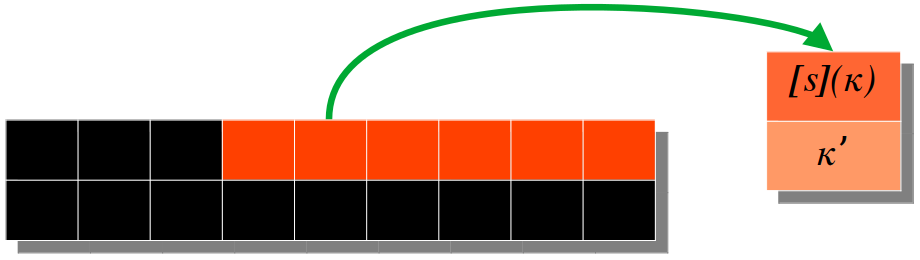
\includegraphics[width=1\linewidth]{conditional}

  \label{fig:qafny-con-analog}
\end{minipage}
\hfill
\begin{minipage}[t]{0.5\textwidth}
\subcaption{Mask/Unmask Function Modeling}
  \begin{mathpar}
    \inferrule[]{R \\ \Omega;\sigma;\varphi\models \theta \mapsto \sch{m}{z_j}{c_{j2}\,|c_{j1}\,\beta_j}}
          {\Omega;\sigma;\varphi\models \mathpzc{M}(b,\theta) 
              \mapsto \sch{m}{z_j}{c_{j1}.c_{j2}\,\beta_j}+q(\kappa,\neg b) }

    \inferrule[]{R
            \\\Omega;\sigma,\varphi\models \theta \mapsto \sch{m'}{z'_j}{c_{j1}.c'_{j2}\,\beta_j}+q(\kappa,\neg b)}
          {\Omega;\sigma,\varphi\models \mathpzc{U}(\neg b,\theta) \mapsto \sch{m}{z_j}{c_{j1}.c_{j2}\,\beta_j}+q(\kappa,\neg b)
  \\\\ \\ * \mathpzc{U}(b,\theta) \mapsto \sch{m'}{z'_j}{c'_{j2}\,|c_{j1}\,\beta_j} }
  \end{mathpar}

  \label{fig:qafny-mu-model}
\end{minipage}

{\begin{minipage}[t]{\textwidth}
\subcaption{Semantic/Proof Rules}
  \begin{mathpar}

\inferrule[SIF]{ R \\ FV(\emptyset,s)\subseteq \kappa'
          \\(\varphi[\kappa'\mapsto \sch{m}{z_j}{c_{j2}\,|c_{j1}\,\beta_j}],s) 
      \longrightarrow (\varphi[\kappa'\mapsto \sch{m'}{z'_j}{c'_{j2}\,|c_{j1}\,\beta_j}],s') } 
{(\varphi[\kappa\uplus\kappa'\mapsto \sch{m}{z_j}{c_{j1}.c_{j2}\,\beta_j}+q(\kappa,\neg b)],\sifq{b}{s}) \longrightarrow 
          (\varphi[\kappa\uplus\kappa'\mapsto \sch{m'}{z'_j}{c_{j1}.c'_{j2}\,\beta_j}+q(\kappa,\neg b)],\sifq{b}{s'}) }

    \inferrule[PIF]{\Omega;\{\kappa' : \tcht\} \vdash Q' \\ \fivepule{\Omega}{\sigma[\kappa' \mapsto \tcht]}{\mmode}{P[\mathpzc{M}(b,\kappa')/ \kappa \uplus \kappa']}{s}{Q * Q'}}
                {\fivepule{\Omega}{\sigma[\kappa \uplus \kappa' \mapsto \tcht]}{g}{P}{\sifq{b}{s}}{P[\mathpzc{U}(\neg b,\kappa \uplus \kappa')/\kappa \uplus \kappa')] * Q'[\mathpzc{U}(b,\kappa \uplus \kappa')/\kappa']}}

\mprset{flushleft}
    \inferrule[SLOOP]{ n_1 < n_2 }
                  {(\varphi,\sqwhile{j}{n_1}{n_2}{b}{s}) \longrightarrow \\\\ \quad (\varphi,\sseq{\sifq{b}{s}}{\sqwhile{j}{\texttt{S}\;n_1}{n_2}{b}{s})}}

    \inferrule[PLOOP]{n_1 < n_2\\ \fivepule{\Omega}{\sigma}{\mmode}{P(j)\wedge j \,\slt\, n_2}{\sifq{b}{s}}{P(\snext{j})} }
     {\fivepule{\Omega}{\sigma}{g}{P(n_1)}{ \sqwhile{j}{n_1}{n_2}{b}{s} }{P(n_2)} }

  \end{mathpar}

  \label{fig:qafny-mu-rules}
\end{minipage}
}
}
{\footnotesize
\[
\begin{array}{l}
\theta := q \mid \kappa
\\[0.2em]
q(\kappa,\neg b) = \schk{m}{z_k}{c_{k1}.c_{k2}\,\beta_k}
\;\;\texttt{where}\;\forall k.\;\slen{c_{k1}}=\slen{\kappa}\wedge \denote{\neg b[c_{k1}/\kappa]}
\\[0.2em]
R = FV(\emptyset,b)=\kappa \wedge \forall j.\; \slen{c_{j1}}=\slen{\kappa}\wedge\denote{b[c_{j1}/\kappa]}
\end{array}
\]
}
\caption{Semantic and Proof Rules for Conditionals and For-loops. $\theta$ is either a session or a quantum state. $\mathpzc{M}$ is the mask function and $\mathpzc{U}$ is the unmask function. }
\label{fig:exp-proofsystem-3}
\end{figure*}

\myparagraph{Rules for Conditionals and For-Loops}\label{sec:conditionals}
\Cref{fig:qafny-con-analog} describes the analogy of quantum conditionals in \qafny, which are partial map functions that only apply applications on the marked red parts and mask the marked black parts.
It contains two level of masking. For each basis state element in a state with session $\kappa_b\uplus \kappa_a$, it masks the $\kappa_b$ part of the state, i.e., if the state has the form: $\sch{m}{z_j}{c_{j1}.c_{j2}\beta_j}$ with $\slen{c_{j1}} = \slen{\kappa_b}$, we mask the $c_{j1}$ part by pushing it to a masked stack as $\sch{m}{z_j}{c_{j2}\,|\,c_{j1}\,\beta_j}$, which is described in preparing the pre-state of the upper-level transition in rule \textsc{SIF} (\Cref{fig:qafny-mu-rules}).
The second level of masking happens in selecting elements in the state by checking the Boolean condition $b$ on them.
The $R$ condition in rule\textsc{SIF} finishes such task for us.
Here, we split the state into two parts as $\sch{m}{z_j}{c_{j1}.c_{j2}\,\beta_j}+q(\kappa,\neg b)$, where the first part are all basis states satisfying $b$ since if we replace the variables in $b$ with $c_{j1}$, the evaluation $\denote{b[c_{j1}/\kappa]}$ returns true, while the second part $q(\kappa,\neg b)$ contains all basis states evaluated to false.
After the masking, we apply the application $s$ on each element in the selected states, install the results ($z'_j$ and $c'_{j2}$ back to the unmasked state, and result in $\sch{m'}{z'_j}{c_{j1}.c'_{j2}\,\beta_j}+q(\kappa,\neg b)$.
The result state number $m'$ might be different from the pre-state number $m$ because applications in $s$ might increase the state numbers such as applying a quantum diffusion operation.

To design a proof rule for such partial map, we develop the mask ($\mathpzc{M}$) and unmask ($\mathpzc{U}$) operations (\Cref{fig:qafny-mu-model}), both take a Boolean expression $b$ and a quantum state as the argument. $\mathpzc{M}$'s modeling materializes the masking mechanism above. For a state $\sch{m}{z_j}{c_{j1}.c_{j2}\,\beta_j}+q(\kappa,\neg b)$, we preserve the basis states satisfying $b$, as shown in the predicate $R$, remove the unsatisfied basis states $q(\kappa,\neg b)$, and push the bases $c_{j1}$ to state stacks.
Here, we do not need to input $\mathpzc{M}$ the session associated with $c_{j1}$, because we can learn it through $b$.
In the pre-condition manipulation of rule \textsc{PIF} (\Cref{fig:qafny-mu-rules}), we substitute $\kappa \uplus \kappa'$ with $\mathpzc{M}(b,\kappa')$. During the process, the type for the session in $\sigma$ is changed from $\kappa \uplus \kappa'$ in the bottom to $\kappa'$ in the upper level.
The unmask function $\mathpzc{U}$ assembles the result state of applying $s$ to the masked $\kappa$ state with the other parts hidden in the unmasked state (the part marked black in \Cref{fig:qafny-con-analog}). Function $\mathpzc{U}$ is usually appeared to be a pair with both $b$ and $\neg b$. In the post-condition manipulation, we substitute $\kappa \uplus \kappa'$ with $\mathpzc{U}(\neg b,\kappa \uplus \kappa')$ in $P$, representing the unchanged and masked state, substitute $\kappa'$ with $\mathpzc{U}(b,\kappa \uplus \kappa')$ in $Q'$, representing the result of applying $s$ on the unmasked part, and assemble them together through the separation operation $*$.
$\mathpzc{U}$'s modeling in \Cref{fig:qafny-mu-model} captures the assemble procedure by merging two $\mathpzc{U}$ constructs together.

Rules \textsc{SLOOP} and \textsc{PLOOP} are the semantic and proof rules for a for-loop, which is a repeat operation of conditionals in \qafny. The $P(j)$ is a loop invariant with $j$ being a variable. The case for $n_1 \ge n_2$ is given in \Cref{sec:newtype}. As an example, we show the proof for a loop-step in \Cref{fig:shorqafny}.

{\footnotesize
  \begin{mathpar}
\mprset{flushleft}
\inferrule[]{
   \inferrule[]
   { \inferrule[] {
    \fivepule{\Omega}{\sigma_2}{\mmode}{X(\snext{j}) * \{y[0..n]\}\mapsto C(j).1}{ s }{X(\snext{j}) * \{y[0..n]\}\mapsto C'(j).1} }
  { \fivepule{\Omega}{\sigma_2}{\mmode}{X(\snext{j}) * \mathpzc{M}(b,\{y[0..n]\})\mapsto 0.C(j)+1.C(j)}{ s }{X(\snext{j}) * \{y[0..n]\}\mapsto C'(j).1} } }
   {  \Omega,\sigma_1\vdash_{\mmode} \{X(\snext{j}) * \{x[0..\snext{j}],y[0..n]\}\mapsto 0.C(j)+1.C(j)\} \sifq{x[j]}{s}
     \\\\\qquad\qquad \{ X(\snext{j}) * \mathpzc{U}(\neg x[j],\{x[0..\snext{j}],y[0..n]\})\mapsto 0.C(j)
          * \mathpzc{U}(x[j],\{x[0..\snext{j}],y[0..n]\})\mapsto C'(j).1\}
     } } {
\fivepule{\Omega}{\sigma}{\mmode}{X(j) * \{x[0..j],y[0..n]\}\mapsto C(j)}{ \sifq{x[j]}{s} }{X(j\,\sminus\,1) * \{x[0..\snext{j}],y[0..n]\} \mapsto 0.C(j)+1.C'(j)} }
  \end{mathpar}
{\hspace*{-1.5em}
$\begin{array}{l}
X(j)=\shad{2^{n \,\sminus\,  j}}{n \,\sminus\, j}{}
\quad
C(j)=\sch{2^k}{\frac{1}{\sqrt{2^k}}}{\tos{j}^{k}.\tos{a^{\tos{j}^k}\;\%\;N}}
\quad
i.C(j)=\sch{2^{\snext{k}}}{\frac{1}{\sqrt{2^{\snext{k}}}}}{\tos{j}^k.i.\tos{a^{\tos{j}^k}\;\%\;N}}
\\
C'(j).i=\sch{2^{\snext{k}}}{\frac{1}{\sqrt{2^{\snext{k}}}}}{\tos{a^{\tos{j}^k.1}\;\%\;N}\,|\,\tos{j}^k.i}
\qquad
i.C'(j)=\sch{2^{\snext{k}}}{\frac{1}{\sqrt{2^{\snext{k}}}}}{\tos{j}^k.i.\tos{a^{\tos{j}^k.1}\;\%\;N}}
\\
\sigma_1=\{x[0..n\,\sminus\,\snext{j}] \mapsto \thadt, \{x[0..\snext{j}],y[0..n]\} \mapsto \tcht \}
\quad
\sigma=\{x[0..n\,\sminus\,\snext{j}] \mapsto \thadt, y[0..n] \mapsto \tcht \}
\quad
s=\ssassign{y}{}{a^{2^j}y\;\%\; N}
\end{array}$
}
}

The proof is built from bottom up. We first cut the $\thadt$ type state into two sessions ($x[0..n\,\sminus\,\snext{j}]$ and $x[j]$), join $x[j]$ with session $\{x[0..j],y[0..n]\}$, and double the state elements to be $0.C(j)+1.C(j)$, which is proved by applying the consequence rules. Notice that the type environment is also transitioned from $\sigma$ to $\sigma_1$.
By the same strategy of the $\mathpzc{U}$ rule in \Cref{fig:qafny-mu-model}, we combine the two $\mathpzc{U}$ terms into the final result. 
The second step applies rule \textsc{PIF} to substitute session $\{x[0..\snext{j}],y[0..n]\}$ with the mask construct $\mathpzc{M}(b,\{y[0..n]\})$ in the pre-condition and create two $\mathpzc{U}$ terms in the post-condition. The step on the top applies the modulo multiplication on every element in the masked state $\mapsto C(j).1$ by rule \textsc{PA-CH}.

\begin{figure*}[t]
{\footnotesize
\begin{minipage}[t]{0.4\textwidth}
\subcaption{Measurement Analogy}
  \vspace{0.5cm}
  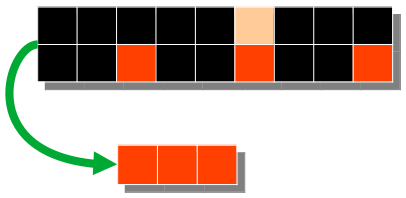
\includegraphics[width=1\linewidth]{measure}

  \label{fig:qafny-mea-analog}
\end{minipage}
\hfill
\begin{minipage}[t]{0.5\textwidth}
\subcaption{Measurement Modeling}
  \begin{mathpar}
    \inferrule[]{\Omega;\sigma;\varphi\models \theta \mapsto \theta'}
          {\Omega;\sigma;\varphi\models \mathpzc{F}(x,n,\theta) \mapsto \mathpzc{F}(x,n,\theta') }

    \inferrule[]{\slen{c}=n \\
           \Omega;\sigma;\varphi\models \theta \mapsto 
                      \sch{m}{\frac{z_j}{\sqrt{r}}}{c_{j}} \wedge x = (r,\tov{c})}
          {\Omega;\sigma,\varphi\models \mathpzc{F}(x,n,\theta) \mapsto \sch{m}{z_j}{c.c_{j}}+q(n,\neq c) }
  \end{mathpar}

  \label{fig:qafny-mea-model}
\end{minipage}

{\begin{minipage}[t]{\textwidth}
\subcaption{Semantic/Proof Rules}
  \begin{mathpar}

    \inferrule[SMea]{\varphi(y) = \{y[0..n]\uplus\kappa\mapsto \sch{m}{z_j}{c.c_{j}}+q(n,\neq c)\}}{(\varphi,\sexp{x}{\smea{y}}{s}) \longrightarrow (\varphi[\kappa \mapsto  \sch{m}{\frac{z_j}{\sqrt{r}}}{c_{j}}],s[(r,\tov{c})/x]) }

    \inferrule[PMea]{\fivepule{\Omega[x\mapsto \mmode]}{\sigma[\kappa\mapsto \tcht]}{\cmode}{P[\mathpzc{F}(x,n,\kappa)/y[0,n]\uplus\kappa]}{s }{Q} }
     {\fivepule{\Omega[y\mapsto \qmode{n}]}{\sigma[y[0,n]\uplus\kappa\mapsto \tcht]}{\cmode}{P}{\sexp{x}{\smea{y}}{s} }{Q} }

  \end{mathpar}

  \label{fig:qafny-mea-rules}
\end{minipage}
}
}
{\footnotesize
\[r= \sum_{k=0}^{m} \slen{z_k}^2
\qquad\qquad
q(n,\neq c) = \schk{m'}{z'_k}{c'.c'_{k}} \;\;\texttt{where}\;c'\neq c\]
}
\caption{Semantic and Proof Rules for Measurement. $\mathpzc{F}$ is the measurement function construct. $\tov{c}$ turns bitstring $c$ to an integer, and $r$ is the likelihood that the bitstring $c$ appears in a basis state. }
\label{fig:exp-proofsystem-4}
\end{figure*}

\myparagraph{Rules for Measurement}\label{sec:measurement}
As \Cref{fig:qafny-mea-analog} describes, quantum measurement is a two-step array filter: 1) each element in the state is partitioned into two parts, and we select a first part of an element as a key, as shown in the marked pink part; and 2) we create a new array state by removing all the first parts in the old state and collecting the elements whose first part is equal to the key.
The second step actually collects elements in a periodical manner as shown in the analogy in \Cref{fig:qafny-mea-analog}, where the marked red basis states appear in a periodical pattern in the whole state. This behavior is universally true for quantum operations, and many quantum algorithms utilize the periodical pattern of quantum computation.

In rule \textsc{SMea}, we pick an $n$-length bitstring $c$ as the marked pink key, and elect $m$ basis states $\sch{m}{z_j}{c.c_{j}}$ that has the key $c$. In the post-state, we update the remaining session $\kappa$ to $\sch{m}{\frac{z_j}{\sqrt{r}}}{c_{j}}$ with the adjustment of amplitude $\frac{1}{\sqrt{r}}$, and replace the variable $x$ in the statement $s$ with the value $(r,\tov{c})$.
In designing the proof rule \textsc{PMea}, the operation $\mathpzc{F}(x,n,\kappa)$ is invented,
whose modeling is in \Cref{fig:qafny-mea-model}, to do exactly the two steps above by selecting an $n$-length prefix bitstring $c$ in a basis state, computing the probability $r$, and assigning $(r,\tov{c})$ to variable $x$.
Rule \textsc{PMea} in \Cref{fig:qafny-mea-rules} replaces the session $y[0..n]\cup \kappa$ in $P$ with the measurement result session $\mathpzc{F}(x,n,\kappa)$ and updates the type state $\Omega$ and $\sigma$. 

{\footnotesize
  \begin{mathpar}
\inferrule[]{
   \inferrule[]
   { \fivepule{\Omega[u\mapsto \mmode]}{\sigma[\kappa \mapsto \tcht]}{\mmode}{\mathpzc{F}(u,n,x[0..n])\mapsto C'}{ \{\} }{x[0..n] \mapsto D * E} }
   { \fivepule{\Omega}{\sigma}{\mmode}{\{y[0..n],x[0..n]\}\mapsto C'}{ \sexp{u}{\smea{y}}{\{\}} }{x[0..n] \mapsto D * E}
     } } {\fivepule{\Omega}{\sigma}{\mmode}{\{x[0..n],y[0..n]\}\mapsto C}{ \sexp{u}{\smea{y}}{\{\}} }{x[0..n] \mapsto D * E} }
  \end{mathpar}
{\hspace*{-1em}
$\begin{array}{l}
C=\sch{2^{n}}{\frac{1}{\sqrt{2^{n}}}}{\tos{j}.\tos{a^{j}\;\%\;N}}
\quad
C'=\sch{2^{n}}{\frac{1}{\sqrt{2^{n}}}}{\tos{a^{j}\;\%\;N}.\tos{j}}
\quad
\sigma=\{\{x[0..\snext{j}],y[0..n]\}:\tcht\}
\\
D=\smch{\frac{1}{\sqrt{s}}}{s}{t\,\splus\,k p}
\quad
E=p = \texttt{ord}(a,N)
\wedge
u=(\frac{s}{2^n},a^{t}\;\%\;N)
\wedge
s=\texttt{rnd}(\frac{2^n}{p})
\end{array}$
}
}

For an instance, we show a proof fragment above for the partial measurement in line 11 in \Cref{fig:shorqafny}.
The bottom two lines are to modify the array group order of the session from 
$\{y[0..n],x[0..n]\}$ to $\{x[0..n],y[0..n]\}$ through the consequence rule of state equivalence.
The second line proof, applies rule $\textsc{PMea}$ by replacing session $\{x[0..n],y[0..n]\}$ with $\mathpzc{F}(u,n,x[0..n])$.
On the top statement, the pre- and post-conditions are equivalent, because of the periodical aspects in quantum computing.
In session $\{y[0..n],x[0..n]\}$, group $y[0..n]$ stores the basis state $\tos{a^{j}\;\%\;N}$, which contains value $j$ that represents the basis states for group $x[0..n]$. Selecting a basis state $a^{t}\;\%\;N$ also filters the $j$ in $x[0..n]$, which refers to any values $j$ having the relation $a^{j}\;\%\;N=a^{t}\;\%\;N$. Notice that modulo multiplication is a periodical function, which means that the relation can be rewritten $a^{t+kp}\;\%\;N=a^{t}\;\%\;N$, such that $p$ is the period order. Thus, the $x[0..n]$ state is rewritten as a summation of $k$: $\smch{\frac{1}{\sqrt{s}}}{s}{t\,\splus\,k p}$. The probability of selecting $\tos{a^{j}\;\%\;N}$ is $\frac{s}{2^n}$.
In \qafny, we set up additional axioms for representing these periodical manners, which is why the pre- and post-condition equivalence is granted.

\begin{figure*}[t]
{\footnotesize
\begin{minipage}[t]{0.35\textwidth}
\subcaption{Diffusion Analogy}
  \vspace{0.5cm}
  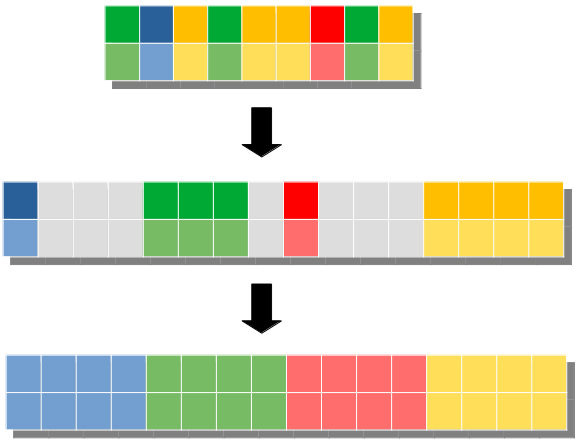
\includegraphics[width=1\linewidth]{diffuse}

  \label{fig:qafny-dis-analog}
\end{minipage}
\hfill
\begin{minipage}[t]{0.6\textwidth}
\subcaption{Diffusion Modeling}
  \begin{mathpar}
    \inferrule[]{\Omega;\sigma;\varphi\models \theta \mapsto \theta'}
          {\Omega;\sigma;\varphi\models \mathpzc{D}(n,\theta) \mapsto \mathpzc{D}(n,\theta') }

    \inferrule[]{\Omega;\sigma;\varphi\models \theta\mapsto \mathpzc{D'}(n,\sch{n'}{z_{i}}{c_{i}})}
          {\Omega;\sigma;\varphi\models \mathpzc{D}(n,\theta) \mapsto \schii{n'}{z_{i}}{c_{i}} }

    \inferrule[]{\slen{\tos{j}}=n
   \\ \Omega;\sigma;\varphi\models \theta\mapsto \Msum_{j=0}^{m}\schk{2^n}{(2 z_{jk}\sum_{t=0}^{2^n}z_{jt} - z_{jk})}{\tos{k}.c_{jk}}}
          {\Omega;\sigma;\varphi\models \theta \mapsto \mathpzc{D'}(n,\Msum_{j=0}^{m}\schk{2^{n}}{z_{jk}}{\tos{k}.c_{jk}}) }
  \end{mathpar}

  \label{fig:qafny-dis-model}
\end{minipage}

{\begin{minipage}[t]{\textwidth}
\subcaption{Semantic/Proof Rules}
  \begin{mathpar}

    \inferrule[SDis]{FV(\Omega,l)=\kappa \\ \varphi(\kappa) = \{\kappa\uplus\kappa'\mapsto q\}}
      {(\varphi,\ssassign{l}{}{\sdis}) \longrightarrow (\varphi[\kappa\uplus\kappa' \mapsto \mathpzc{D}(\slen{\kappa},q)],\{\}) }

    \inferrule[PDis]{ FV(\Omega,l)=\kappa\\\sigma(\kappa)=\{\kappa\uplus\kappa:\tcht\} }
     {\fivepule{\Omega}{\sigma}{g}{P[\mathpzc{D}(\slen{\kappa},\kappa\uplus\kappa')/\kappa\uplus\kappa']}{\ssassign{l}{}{\sdis} }{P} }

  \end{mathpar}

  \label{fig:qafny-dis-rules}
\end{minipage}
}
}
\caption{Semantic and Proof Rules for Diffusion Operations. $\mathpzc{D}$ models the diffusion operations. }
\label{fig:exp-proofsystem-5}
\end{figure*}

\myparagraph{Rules for Diffusion}\label{sec:diffuse}
Quantum diffusion operations ($\ssassign{l}{}{\sdis}$) reorient the amplitudes of basis states based on the basis state corresponding to $l$. They are analogized to an aggregate operation of reshape and mean computation, both appeared in many programming languages \footnote{Such as Python}.
The aggregate operation first applies a reshape, where elements are regrouped into a normal form, as the first agree of \Cref{fig:qafny-dis-analog}. More specifically, the diffusion modeling function $\mathpzc{D}(n,\theta)$ takes an $n'$-element state $\sch{n'}{z_{j}}{c_{j}}$ as the second rule in \Cref{fig:qafny-dis-model}. The $n$ number corresponds to the number of bits in the session potion matching $l$.
Then, we rearrange the state by a helper function $\mathpzc{D'}$ by extending the element number from $n'$ to $m*n$ with probably adding new elements that originally have zero amplitude (the marked white elements in \Cref{fig:qafny-dis-analog}), as the third rule in \Cref{fig:qafny-dis-model}.
Here, let's view a basis $c_{i}$ as a small-endian (LSB) number $\tov{c_{i}}$. The rearrangement of changing bases $c_{i}$ (for all $i$) to $\tos{k}.c_{jk}$ is analogized to rearranging a number $\tov{c_{i}}$ to become the form $2^n j+k$, with $k\in [0,2^n)$. 
Basically, the reshape step rearranges the basis states to be placed in a periodical counting sequence, with $2^n$ being the order.

The mean computation analogy (the second arrow in \Cref{fig:qafny-dis-analog}) takes every period in the reshaped state, and for each basis state, we redistribute the amplitude by the formula $(2 z_{jk}\sum_{t=0}^{2^n}z_{jt} - z_{jk})$.
In another word, for each period, given a basis state $k$, we sum all the amplitudes from $0$ to $2^n$ in the period as $z_{sum}$, then the redistributed amplitude for $k$ is $2 z_k z_{sum}-z_k$. 

Rule \textsc{SDis} is the semantics for diffusion $\ssassign{l}{}{\sdis}$, which applies the $\mathpzc{D}$ function to the session $\kappa \uplus \kappa'$, where $\kappa$ corresponds to the $l$'s session. Proof rule \textsc{PDis} replaces session $\kappa\uplus \kappa'$ with the application $\mathpzc{D}$ on the session.
Quantum diffusion operations are used in many algorithms, such as amplifying a basis state's amplitude value in Grover's search algorithm, or redistributing a possible path direction in quantum walk algorithm.
In these algorithms, the session piece that is diffused has either a small constant number of qubits or the whole session, meaning that the $n$ number in the $\mathpzc{D}$ function is either very small or equal to $\slen{\kappa \uplus \kappa'}$, as the whole session.
In either case, the summation formula in $\mathpzc{D}$'s modeling (\Cref{fig:qafny-dis-model}) can be rewritten as very few terms that facilitate the automated verification, which is exactly how we handle the diffusion operations in \qafny.
An example of Grover's search and quantum walk algorithm is given in \Cref{sec:arith-oqasm}.

\subsection{\qafny Metatheory}\label{sec:theorems}

The type system is sound and the proof system is proved to be sound and complete.


\myparagraph{Type Soundness}
We prove that well-typed \qafny programs are well defined; i.e., the
type system is sound with respect to the semantics. 
We begin by defining the session domain and state well-formedness.





The \qafny type soundness is stated as two theorems, type progress and preservation theorems. The proofs are done by induction on \qafny statements $s$ and mechanized in Coq. Type progress states that any well-typed \qafny program can take a move, while type preservation states that for any such move, the transitioned type and state are preserved and well-typed, respectively.

\begin{theorem}[\qafny type progress]\label{thm:type-progress-oqasm}\rm 
If $\Omega;\sigma \vdash_g s \triangleright \sigma'$ and $\Omega;\sigma \vdash \varphi$, then either $s=\{\}$, or there exists $\varphi'$ and $s'$ such that $(\varphi,s)\longrightarrow (\varphi',s')$.
\end{theorem}

\begin{theorem}[\qafny type preservation]\label{thm:type-preservation-oqasm}\rm 
If $\Omega;\sigma \vdash_g s \triangleright \sigma'$, $\Omega;\sigma \vdash \varphi$, and $(\varphi,s)\longrightarrow (\varphi',s')$, then 
there exists $\Omega'$ and $\sigma''$, $\Omega';\sigma'' \vdash_g s' \triangleright \sigma'$ and $\Omega';\sigma'' \vdash \varphi'$.
\end{theorem}

\myparagraph{Proof System Soundness and Completeness}
We prove that the \qafny proof system is well defined; i.e., any properties derived in the \qafny proof system for well-typed \qafny programs can be interpreted by the state transitions in the \qafny semantics.
In \qafny, there are three different state representations for a session $\kappa$ and two sessions can be joined into a large session.
Hence, given a statement $s$ and an initial state $\varphi$, the semantic transition $(\varphi,s) \longrightarrow^{*} (\varphi',\{\})$ might not be unique, in the sense that there might be different representations of $\varphi'$, due to the different state representations.
However, any $\tnort$ and $\thadt$ type state can be represented as a $\tcht$ type state, so that $\tcht$ type states can be viewed as the \emph{most general} state representation. We also have state equivalence relations defined for capturing the behaviors of session permutation, join and split. We define a \emph{most general state representation} of evaluating a statement $s$ in an initial state $\varphi$ below.

\begin{definition}[Most general \qafny state]\label{def:most-gen}\rm 
  Given a statement $s$, an initial state $\varphi$, kind environment $\Omega$, type environment $\sigma$, and context mode $g$, such that $\Omega;\sigma\vdash \varphi$, $\vdash_g s \triangleright \sigma^*$, $\Omega;\sigma[\uparrow \sigma^*]\vdash \varphi^*$, and $(\varphi,s) \longrightarrow^{*} (\varphi^*,\{\})$, $\varphi^*$ is the most general state representation of evaluating $(\varphi,s)$, iff for all $\sigma'$ and $\varphi'$, such that $\vdash_g s \triangleright \sigma'$, $\Omega;\sigma[\uparrow \sigma']\vdash \varphi'$ and $(\varphi,s) \longrightarrow^{*} (\varphi',\{\})$, $\sigma' \preceq \sigma^*$ and $\varphi' \equiv \varphi^*$.
\end{definition}

The \qafny proof system correctness is defined by the soundness and relatively completeness theorems below, which has been formalized and proved in Coq. The \qafny proof system only describes the quantum portion of the whole Qafny+Dafny system, and the quantum portion contains non-terminated programs. Hence, the soundness and completeness essentially refers to the partial correctness of the \qafny proof system and the total correctness is achieved by the Qafny+Dafny system through mapping \qafny to Dafny, i.e., a separation logic proof system. Essentially, the \qafny proof system correctness is defined in terms of programs being well-typed. The type soundness theorem suggests that any intermediate transitions of evaluating a well-typed \qafny program is also well-typed. Thus, we can conclude that the pre- and post- conditions of a program are modeled properly through the above modeling rules that rely on well-typed transition states.

\begin{theorem}[proof system soundness]\label{thm:proof-soundness}\rm 
For a well-typed program $s$, such that $\Omega;\sigma\vdash_g s \triangleright \sigma'$, $\fivepule{\Omega}{\sigma}{g}{P}{s}{Q}$, $\Omega;\sigma;\varphi\models P$, then there exists a state representation $\varphi'$, such that $(\varphi,s)\longrightarrow (\varphi',\{\})$ and $\Omega;\sigma[\uparrow\sigma'];\varphi'\models Q$, and there is a most general state representation $\varphi^*$ of evaluating $(\varphi,s)$ as $(\varphi,s)\longrightarrow (\varphi^*,\{\})$ and $\varphi' \equiv \varphi*$.
\end{theorem}

\begin{theorem}[proof system relative completeness]\label{thm:proof-completeness}\rm 
For a well-typed program $s$, such that $\Omega;\sigma\vdash_g s \triangleright \sigma'$, $(\varphi,s)\longrightarrow (\varphi',\{\})$ and $\Omega;\sigma\vdash \varphi$, there is most general state representation $\varphi^*$, such that $(\varphi,s)\longrightarrow (\varphi',\{\})$ and $\varphi' \equiv \varphi^*$ and $\Omega;\sigma\vdash_g s \triangleright \sigma^*$ and $\Omega;\sigma[\uparrow \sigma^*]\vdash \varphi^*$, and there are predicates $P$ and $Q$, such that $\Omega;\sigma;\varphi\models P$ and $\Omega;\sigma[\uparrow\sigma^*];\varphi^* \models Q$ and $\fivepule{\Omega}{\sigma}{g}{P}{s}{Q}$.
\end{theorem}




